\chapter{Stabilità nei sistemi dinamici}


\section{Sistema dinamico e punti di equilibrio}

Un sistema dinamico 
è composta da uno stato \(x \in \mathbb{R}^{n}\)
e da una legge di evoluzione

\begin{equation}
  \dot{x}(t) = f(x(t), u(t), t)
  \label{sistema-dinamico-generale}
\end{equation}

\begin{definizione}
Un sistema è detto \textbf{tempo invariante} se la
  sua evoluzione non dipende esplicitamente dal tempo \(t\), cioè:
  \[\dot{x}(t) = f(x(t), u(t))\]
\end{definizione}


\begin{definizione}
Un sistema è detto \textbf{autonomo} se la sua evoluzione non dipende esplicitamente
  dall'ingresso \(u(t)\), cioè:
  \[\dot{x}(t) = f(x(t),t)\]
\end{definizione}

Se il sistema è sia autonomo che tempo invariante
allora si ha:
\[\dot{x}(t) = f(x(t))\]




\begin{definizione}
Dato un sistema dinamico \textbf{tempo invariante} nella forma:
\[\dot{x}(t) = f(x(t), u(t))\]
un punto di equilibrio \((\bar{x}, \bar{u})\) è una coppia 
stato-ingresso tale che:
\[\dot{x} = f(\bar{x}, \bar{u}) = 0\]


\end{definizione}



\section{Stabilità e Convergenza}



\begin{definizione}

Un punto di equilibrio \(\bar{x}\) di un sistema dinamico 
tempo invariante è detto stabile se:

\begin{equation}
  \forall \varepsilon > 0, 
  \exists \delta > 0 : x_{0} 
  \in B_{\delta}(\bar{x})
  \Rightarrow |x_{x_{0}}(t) - \bar{x}| \le \varepsilon, \forall t \geq 0
  \label{stabilità}
\end{equation}Dove con \(x_{x_{0}}(t)\) si intende 
la traiettoria del sistema 
che parte da \(x_{0}\).
\end{definizione}



Ora dimostriamo che \(\delta \le 
\varepsilon ,
\forall \varepsilon > 0\).
\begin{proof}
  
Supponiamo per assurdo che 
esista un \(\varepsilon >0 \)
per cui si ha  
che la \(\delta\)
per cui è rispettata la 
definizione di stabilità sia
tale che
\(\delta > \varepsilon\).
Allora si ha che per
le 
\(x_{0} \in B_{\delta}(\bar{x}) \backslash
B_{\varepsilon}(\bar{x})\)
vale:
\[|x_{x_{0}}(0) - \bar{x}| 
= \left|x_{0} -\bar{x}\right|> \varepsilon\]
Ma questo è assurdo perché
\(x_{0} 
\in B_{\delta}(\bar{x})\)
dunque rispetta la definizione 
di stabilità per cui
si dovrebbe avere :
\[|x_{x_{0}}(0) - \bar{x}| 
= \left|x_{0} - \bar{x}\right|
\le \varepsilon
\]
Dunque siamo arrivati ad un assurdo.

\end{proof}



\begin{definizione}
  Dato un sistema dinamico un punto di equilibrio
  \(\bar{x}\) è detto \textbf{convergente} se esiste un 
  \(\delta >0\) tale che per ogni condizione iniziale
  \(x_{0} \in B_{\delta}(\bar{x})\) si ha che:
  \[\lim_{t \to \infty} \left|\left|x(t) - \bar{x}\right|\right| = 0\]

\end{definizione}

\begin{definizione}
  Un punto di equilibrio \(\bar{x}\) è detto 
  \textbf{isolato} se esiste un intorno di \(\bar{x}\)
  che non contiene altri punti di equilibrio.
\end{definizione}


% ...existing code...
\begin{figure}[htbp]
  \centering
  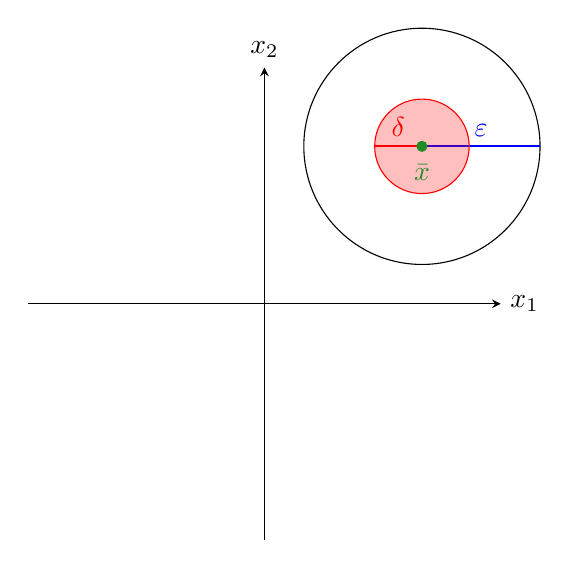
\begin{tikzpicture}[scale=1, >=stealth]
    % assi con sole etichette x1 e x2
    \draw[->] (-3,0) -- (3,0) node[right] {$x_1$};
    \draw[->] (0,-3) -- (0,3) node[above] {$x_2$};


    % cerchio grande e raggio epsilon
    \draw (2,2) circle (1.5);
    \draw[thick, blue] (2,2) -- ++(1.5,0) node[midway, above] {$\varepsilon$};

    % cerchio piu' piccolo rosso trasparente e raggio delta (più corto)
    \filldraw[fill=red, fill opacity=0.25, draw=red] (2,2) circle (0.6);
    \draw[thick, red] (2,2) -- ++(-0.6,-0) node[midway, above] {$\delta$};

    \filldraw[ForestGreen] (2,2) circle (1.8pt) node[below=3pt] {$\bar{x}$};

  \end{tikzpicture}
  \caption{In \textcolor{ForestGreen}{verde} si ha il 
  punto di equilibrio \textcolor{ForestGreen}{\(\bar{x}\)}. 
  In rosso si ha l'insieme delle condizioni iniziali per cui le traiettorie rimangono
  confinate  all'interno del cerchio di raggio \(\varepsilon\).}
  \label{fig:assi-x1-x2}
\end{figure}
% ...existing code...
\section{Stabilità nei sistemi lineari}

Consideriamo un sistema lineare
tempo invariante:
\[\dot{x}(t) = Ax(t) + Bu(t)\]
Dove \(A \in \mathbb{R}^{n \times n}\) e 
\(B \in \mathbb{R}^{n \times m}\).
Per trovare i punti di equilibrio dobbiamo imporre:
\[\dot{x}(t) = 0 \Longleftrightarrow Ax(t) + Bu(t) = 0\]
Dunque i punti di equilibrio 
sono le coppie \((\bar{x}, \bar{u})\) che soddisfano:
\[ 
A\bar{x} + B\bar{u} = 0
\]
Notiamo subito che il punto \((\bar{x}, \bar{u}) = (0,0)\)
 è sicuro un punto di equilibrio.
Mentre gli altri punti si trovano risolvendo il sistema lineare
omogeneo considerando \(\bar{x}\) e \(\bar{u}\) come incognite.
Se invece di considerare le coppie \((\bar{x}, \bar{u})\) di equilibrio
consideriamo solo gli stati di equilibrio \(\bar{x}\) con un 
fissato \(\bar{u}\), allora l'unica incognita è \(\bar{x}\) 
mentre \(B \bar{u}\) è un termine noto.
In questo caso il sistema lineare da risolvere è:
\[A \bar{x} = - B \bar{u}\]
Questo sistema al variare di \(\bar{u}\) 
(che funge da parametro) ammette soluzioni differenti,
però la matrice \(A\) ci dice quante sono queste soluzioni.
Se \(A\) è invertibile (ovvero \(\det(A) \neq 0\))
allora esiste un'unica soluzione per ogni \(\bar{u}\):
\[\bar{x} = -A^{-1}B \bar{u}\]
Se invece \(A\) non è invertibile (ovvero \(\det(A) = 0\))
allora il sistema può ammettere infinite soluzioni oppure nessuna soluzione
(ricordiamo che il sistema si risolve
al variare del parametro \(\bar{u}\)).

\section{Sistema nel dominio di Laplace}
Consideriamo il sistema lineare tempo invariante:
\[\dot{x}(t) = Ax(t) + Bu(t)\]
Applichiamo la trasformata di Laplace ambo i membri otteniamo:
\[sX(s) - x(0) = AX(s) + BU(s)\]
Portando \(x(0)\) a destra e portando \(AX(s)\) a sinistra otteniamo:
\[sX(s) - AX(s) = BU(s) + x(0)\]
Ricordando che \(sX(s) = s I X(s)\) e mettendo in evidenza \(X(s)\) otteniamo:
\[(sI - A)X(s) = BU(s) + x(0)\]
Ora premoltiplichiamo ambo i membri per
\((sI - A)^{-1}\) otteniamo:
\[X(s) = \textcolor{red}{(sI - A)^{-1}BU(s)} + \textcolor{blue}{(sI - A)^{-1}x(0)}\]
Dove in \textcolor{red}{rosso} abbiamo la parte dovuta all'ingresso
che prende il nome di \textcolor{red}{evoluzione forzata}  dello stato, 
mentre in \textcolor{blue}{blu}
abbiamo la parte dovuta alla  \textcolor{blue}{evoluzione libera}
dello stato (che ricordiamo essere nulla se \(x(0) = 0\)).
Andando a fare la stessa cosa per l'equazione di uscita:
\[y(t) = Cx(t) + Du(t)\]
Applichiamo la trasformata di Laplace otteniamo:
\[Y(s) = CX(s) + DU(s)\]
Sostituendo \(X(s)\) otteniamo:
\[Y(s) = C\left[(sI - A)^{-1}BU(s) + (sI - A)^{-1}x(0)\right] + DU(s)\]
Dove riusciamo un'altra volta a distinguere una parte
in \textcolor{red}{evoluzione forzata} ed un una in \textcolor{blue}{
evoluzione libera}:
\[Y(s) =\textcolor{red}{C \left[\left(sI - A\right)^{-1} + D\right]BU(s)} +
\textcolor{blue}{ 
\left(sI - A\right)^{-1}x(0)} \]


\section{Stabilità tramite l'approccio alla Lyapunov}

Ora ci interessa introdurre un metodo per studiare la stabilità
dei sistemi dinamici che prende il nome di \textbf{approccio di Lyapunov},
che ci permette di studiare la stabilità dei sistemi andandoci a 
trovare delle specifiche funzioni 
scalari \(V(x) : 
\mathbb{R}^n \to \mathbb{R}\) dette \textbf{funzioni di Lyapunov}.
Per prima cosa ricordiamo che una funzione \(V(x) : \mathbb{R}^{n} 
\to \mathbb{R}\) e un suo punto di equilibrio 
possono essere classificati come:
\begin{itemize}
  \item \textbf{definita positiva} 
  in \(\bar{x}\) se \(V(\bar{x}) = 0\) ed esiste un \(\delta > 0\)
  tale che \(V(x) > 0\) (notiamo il maggiore stretto) per ogni \(x \in B_{\delta}(\bar{x})\)
  \item \textbf{semidefinita positiva} 
  in \(\bar{x}\) se \(V(\bar{x}) = 0\) ed esiste un \(\delta > 0\)
  tale che \(V(x) \ge 0\) per ogni \(x \in B_{\delta}(\bar{x})\)
  \item \textbf{definita negativa} 
  in \(\bar{x}\) se \(V(\bar{x}) = 0\) ed esiste un \(\delta > 0\)
  tale che \(V(x) < 0\) per ogni \(x \in B_{\delta}(\bar{x})\)
  \item \textbf{semidefinita negativa} 
  in \(\bar{x}\) se \(V(\bar{x}) = 0\) ed esiste un \(\delta > 0\)
  tale che \(V(x) \le 0\) per ogni \(x \in B_{\delta}(\bar{x})\)
\end{itemize}
Queste proprietà diventano \textbf{globali}
quando sono vere per ogni \(\bar{x} \in \mathbb{R}^{n}\).
La potenza del metodo che stiamo per introdurre
sta nel fatto che è valida anche per sistemi non lineari,
nel momento in cui aggiungeremo l'ipotesi di linearità andremo 
ad ottenere anche altri risultati.

\begin{teorema}
Teorema di Lyapunov.  Consideriamo il sistema dinamico:
\[\dot{x}(t) = f(x(t))\]
Consideriamo il punto di equilibrio \(\bar{x}\) per \(f\).
Se \(f\) è definita, è continua ed anche la sua derivata è continua
in un intorno \(D\) di \(\bar{x}\),
cioè \(f \in C^{1}(D)\) (\(f\) 
è un vettore di funzioni quindi quando diciamo che è 
continua intendiamo che ogni sua componente lo è).
Se esiste una funzione \(V(x) : \mathbb{R}^{n} \to \mathbb{R}\), 
continua e derivabile in \(D\), tale che:
\begin{itemize}
  \item \(V(x)\) è definita positiva in \(\bar{x}\), cioè:
  \[\begin{cases}
    V(\bar{x}) = 0 \\
    \exists \delta : V(x) > 0, \quad \forall x \in B_{\delta}(\bar{x}) \backslash \{\bar{x}\}
  \end{cases}\]
  \item \(\dot{V}(x)\) è semidefinita negativa in \(\bar{x}\), cioè:
  \[\begin{cases}
    V(\bar{x}) = 0 \\
    \exists \delta > 0: \dot{V}(x) = \nabla V(x) \cdot 
    \displaystyle 
    \frac{dx}{dt} = \nabla V(x(t)) f(x(t)) \le 0, \quad \forall x \in B_{\delta}(\bar{x}),
    \forall t > t_0 
  \end{cases}\]
\end{itemize}
Allora si ha che il punto di equilibrio \(\bar{x}\) è stabile.
\end{teorema}

\begin{proof}
Noi vogliamo dimostrare che \(\bar{x}\) è un punto di equilibrio stabile,
cioè che per ogni \(\varepsilon > 0\) esiste un \(\delta > 0\)
tale che se \(x_{0} \in B_{\delta}(\bar{x})\) allora
la traiettoria \(x(t)\) che parte da \(x_{0}\)
rimane confinata in \(B_{\varepsilon}(\bar{x})\).
Dunque partiamo con il fissare un generico \(\varepsilon > 0\).
Prendiamo la curva di livello (della funzione \(V(x)\)) 
a valore maggiore e completamente contenuta in \(\bar{B}_{\varepsilon}(\bar{x})\) 
(con il trattino sopra intendiamo la chiusura), come 
in Figura \ref{fig:lyapunov-proof}. Ora chiamiamo \(\delta\)
la distanza minima tra \(\bar{x}\) e la curva di livello di valore \(\bar{V}\).
Ora consideriamo una \(x(t)\)
che parte da un punto \(x_{0} \in B_{\delta}(\bar{x})\) 
\((x(t_{0}) = x_{0})\). A noi interessa dimostrare che \(\bar{x}\) è
stabile, cioè che \(\forall x_0 \in B_{\delta}(\bar{x})\)
la traiettoria \(x(t)\) rimane confinata all'interno di \(B_{\varepsilon}(\bar{x})\)
\(\forall t \ge 0\). Per dimostrare che \(x(t)\) rimane confinata in
\(B_{\varepsilon}(\bar{x})\) distinguiamo due casi:
\begin{itemize}
  \item Nel caso in cui si ha \(\dot{V}(x) = 0\) la traiettoria \(x(t)\) nel peggiore 
  casi rimane confinata sulla curva di livello a valore \(\bar{V}\), o su un'altra 
  curva di livello a valore minore di \(\bar{V}\) (dunque rimane confinata in
  \(B_{\varepsilon}(\bar{x})\)).
  \item  Se  \(\dot{V}(x) < 0\) allora la traiettoria \(x(t)\) si muove 
  in modo tale da far diminuire il valore di \(V(x(t))\), quindi si muove
   verso l'interno   (essendo \(\bar{V}\) la curva di livello a valore massimo)
  della curva di livello a valore \(\bar{V}\) 
  (dunque rimane confinata in \(B_{\varepsilon}(\bar{x})\))
\end{itemize}
Quindi in entrambi i casi la traiettoria \(x(t)\)
rimane confinata in \(B_{\varepsilon}(\bar{x})\). 
Dunque abbiamo dimostrato che per ogni \(\varepsilon > 0\)
esiste un \(\delta > 0\) tale che se \(x_{0} \in B_{\delta}(\bar{x})\)
allora la traiettoria \(x(t)\) rimane confinata in
\(B_{\varepsilon}(\bar{x})\) \(\forall t \ge t_{0}\),
ma questa è proprio la definizione di stabilità. 
\begin{figure}[htbp]
    \centering
    \begin{tikzpicture}[>=stealth, scale=1.3]

        % 1. Parametri geometrici
        \coordinate (XBAR) at (3, 2.5);
        
        % Raggio Epsilon (Cerchio esterno limite)
        \def\Reps{2.5}
        % Raggio Delta (Cerchio interno)
        \def\Rdelta{1.0} 

        % 2. Assi
        \draw[->, thick] (-1, 0) -- (7, 0) node[right] {$x_1$};
        \draw[->, thick] (0, -1) -- (0, 6) node[above] {$x_2$};

        % 3. Centro x_bar
        \fill (XBAR) circle (2pt) node[below left] {$\bar{x}$};

        % 4. Circonferenza Epsilon (Nera - Esterna)
        \draw[thick] (XBAR) circle (\Reps);
        \draw[dashed, ->] (XBAR) -- ++(45:\Reps) node[midway, above left] {$\epsilon$};
        
        % 5. Curva di livello V_bar di forma CASUALE (Blu)
        % Utilizziamo 'plot smooth cycle' definendo dei punti di controllo attorno a XBAR.
        % L'importante è che la distanza di questi punti da XBAR sia sempre < Reps (2.5)
        % Usiamo coordinate polari relative: ([shift=(angolo:raggio)]Centro)
        \draw[blue, thick] plot [smooth cycle, tension=0.7] coordinates {
            ([shift=(0:2.2)]XBAR)   % Est, vicino al bordo
            ([shift=(50:1.5)]XBAR)  % Nord-Est, rientranza
            ([shift=(90:2.1)]XBAR)  % Nord
            ([shift=(140:1.7)]XBAR) % Nord-Ovest
            ([shift=(180:2.3)]XBAR) % Ovest, vicino al bordo
            ([shift=(230:1.6)]XBAR) % Sud-Ovest
            ([shift=(270:1.9)]XBAR) % Sud
            ([shift=(320:1.4)]XBAR) % Sud-Est, rientranza marcata
        };
        % Etichetta V_bar
        \node[blue, right] at ($(XBAR) + (2.2, 0.2)$) {$\bar{V}$};

        % 6. Circonferenza Delta (Rossa - Interna)
        % Contenuta nella curva casuale
        \draw[red, thick] (XBAR) circle (\Rdelta);
        \draw[red, dashed, ->] (XBAR) -- ++(135:\Rdelta) node[midway, right] {$\delta$};

    \end{tikzpicture}
    \caption{Visualizzazione con una curva di livello $\bar{V}$ (blu) di forma generica non ellittica, strettamente contenuta all'interno della circonferenza di raggio $\epsilon$ (nera).}
    \label{fig:livello_casuale}
\end{figure}

\end{proof}


Se \( f \in C^{1}(D) \) allora è anche sicuramente
 localmente Lipschitziana
in  \(D\) (poichè se una funzione è \(C^{1}\) allora 
il suo gradiente è limitato) cioè:
\[\exists L >0  : \|f(x) - f(y)\| \le L \|x - y\|, \quad \forall x,y \in I\] 

\section{Lyapunov per Sistemi LTI}
Per i sistemi lineari tempo invarianti possiamo 
utilizzare il metodo di Lyapunov per studiare l'asintotica stabilità
del sistema. 
Consideriamo il sistema LTI:
\[\dot{x} = Ax + Bu\]
Ricordiamo che per tutti i sistemi linerari l'asintotica stabilità è una proprietà 
del sistema, cioè se un punto di equilibrio è asintoticamente stabile allora lo sono tutti.
Tutti i sistemi LTI ammettono come punto di equilibrio l'origine
\((\bar{x}, \bar{u}) = (0,0)\), 
e quindi possiamo anche andare a studiare direttamente 
la stabilità di questo punto di equilibrio (che ci 
permette di non considerare gli ingressi). Dunque consideriamo direttamente
il sistema autonomo (che si evolve senza ingressi):
\[\dot{x} = Ax\]
Studiamo con il metodo di Lyapunov la stabilità dell'origine (nello spazio 
dello stato e degli ingressi) come 
punto di equilibrio. Per i sistemi LTI vale il seguente teorema:
\begin{teorema}
Teorema di Lyapunov per sistemi LTI. 
Il sistema LTI:
\[\dot{x} = Ax\]
è stabile se e solo se per ogni matrice \(Q \) simmetrica definita positiva (\(Q=Q^{T} > 0\)),
esiste una matrice simmetrica definita positiva \(P=P^{T} > 0\)
tale che:
\begin{equation}  
  A^{T}P + PA = -Q
\end{equation}
quest'ultima equazione prende il nome di \textbf{equazione di Lyapunov}.
\end{teorema}
Dimostriamo il seguente teorema.
\begin{proof}
  Partiamo con il mostrare che l'esistenza di \(P\) 
  che soddisfa l'equazione di Lyapunov è una \textbf{condizione necessaria}
  alla asintotica stabilità. Prendiamo una generica \(Q=Q^{T}>0\), 
  vogliamo dimostrare che supposto il sistema sia asintoticamente stabile, allora deve 
  esistere una \(P=P^{T}>0\) che soddisfa l'equazione di Lyapunov:
  \[  A^{T}P + PA = -Q \]
  Consideriamo la \(P\) definita come:
  \[ P =\int_{0}^{+\infty} e^{A^{T}t} Q e^{At} dt \]
  Per prima cosa diciamo che questa \(P\) è ben definita (l'integrale converge 
  \(\forall Q\)) poichè il sistema è asintoticamente stabile, dunque 
  gli esponenziali che usciranno nei calcoli avranno tutti 
  esponenti negativi, dunque si avrà \(e^{\lambda t} \to 0\) per \(t \to +\infty\)
  (poichè \(\lambda <0 \)).

  Per costruzione questa \(P\) è simmetrica.
  Dimostriamo ora che questa \(P\) è definita positiva. Preso un generico
  \(x \in \mathbb{R}^{n} - \left\{0\right\}\) vogliamo dimostrare che \(x^{T}Px > 0\).
  Calcoliamo:
  \[ x^{T}Px = x^{T} \left( \int_{0}^{+\infty} e^{A^{T}t} Q e^{At} dt \right) x  \]
  Portiamo le \(x\) dentro l'integrale:
  \[ x^{T}Px = \int_{0}^{+\infty} x^{T} e^{A^{T}t} Q e^{At} x dt \]
  Notiamo ora che a primo membro abbiamo \(x^{T} e^{A^{T} t} = \left(e^{At} x\right)^{T}\):
  \[ x^{T}Px = \int_{0}^{+\infty} \left(e^{At} x\right)^{T} Q \left(e^{At} x\right) dt\]
  Ora poniamo \(y = e^{At}x\), ci interessa dimostrare che:
  \[ \int_{0}^{+\infty} y^{T} Q y dt > 0 \]
  Ora noi sappiamo che \(Q\) è definita positiva,
  dunque per definizione di matrice definita positiva si ha che:
  \[ y^{T} Q y > 0 ,  \forall y \neq 0 \]
  Il nostro problema è diventato dunque dimostrare che \(y \neq 0\) per ogni
  \(x \neq 0\). Ricordiamo che l'esponenziale di 
  matrice è sempre invertibile, dunque la dimensione del \(ker(e^{At})\) è nulla,
  quindi \(y =e^{At}x \neq 0 \forall x \neq 0\). Dunque abbiamo dimostrato che:
  \[ y^{T} Q y > 0 ,  \forall x \neq 0 \]
  Quindi abbiamo dimostrato che l'integrando è sempre positivo per ogni \(t \ge 0\).
  Ma se l'integrando è sempre positivo anche l'intergrale è
  positivo dunque la matrice \(P\) è definita positiva.
  Ora dimostriamo che questa \(P > 0\) soddisfa l'equazione di Lyapunov.
  Calcoliamo:
  \[A^{T} P + P A = 
  A^{T} \int_{0}^{+\infty} e^{A^{T}t} Q e^{At} dt  +
  \int_{0}^{+\infty} e^{A^{T}t} Q e^{At} dt  A\] 
  Portando \(A^{T}\) e \(A\) dentro gli integrali, 
  ed unendo gli integrali otteniamo:
    \[A^{T} P + P A = 
  \int_{0}^{+\infty}
  A^{T} 
  e^{A^{T}t} Q e^{At} dt  +
  e^{A^{T}t} Q e^{At} dt  
  A\] 
  Ora notiamo che il termine all'interno dell'integrale
  è la derivata di \(e^{A^{T}t} Q e^{At}\) rispetto a \(t\), dunque possiamo riscrivere:
  \[A^{T} P + P A =  
  \int_{0}^{+\infty} \frac{d}{dt} \left( e^{A^{T}t} Q e^{At} \right) dt
  \]
  Ma l'integrale della derivata è proprio la funzione valutata agli estremi:
  \[ 
  A^{T} P + P A= \left[ e^{A^{T}t} Q e^{At} \right]_{0}^{+\infty}
  \]
  Ma \[e^{A^{T}t} Q e^{At}\] valutata in \(0\) vale \(Q\), mentre
  valutata in \(+\infty\) vale \(0\) (poichè il sistema è asintoticamente stabile),
  dunque si ha:
  \[ A^{T} P + P A = 0 - Q = -Q\]
  Dunque abbiamo dimostrato che se il sistema è asintoticamente stabile
  allora per ogni \(Q=Q^{T} > 0\) esiste una \(P=P^{T} > 0\)
  che soddisfa l'equazione di Lyapunov. \\
  Ora dimostriamo la \textbf{condizione sufficiente}, cioè
  se \(\forall Q=Q^{T} >0\) esiste una \(P=P^{T} > 0\) che soddisfa l'equazione di Lyapunov
  allora il sistema è asintoticamente stabile.
  Per ipotesi dunque sappiamo che fissata una \(Q=Q^{T} > 0\) 
  esiste almeno una \(P=P^{T} > 0\) che soddisfa l'equazione di Lyapunov,cioè:
  \[ A^{T} P + P A = -Q \]
  Il nostro obiettivo è dimostrare che il sistema è asintoticamente stabile,
  dunque andiamo a considerare la funzione di Lyapunov:
  \[ V(x) = x^{T} P x \]
  Noi sappiamo che \(P\) è definita positiva, dunque \(V(x)\) è definita positiva.
  Calcoliamo ora la derivata di \(V(x)\) lungo
  le traiettorie del sistema (ricordiamo la regola 
  della derivata di una forma quadratica):
  \[ \dot{V}(x) = \dot{x}^{T} P x + x^{T} P \dot{x} \]
  Ricordiamo che \(\dot{x} = Ax\), dunque sostituiamo:
  \[ \dot{V}(x) = (Ax)^{T} P x + x^{T} P (Ax) \]
  Facendo il trasposto a primo membro:
  \[ \dot{V}(x) = x^{T} A^{T} P x + x^{T} P A x \]
  Mettiamo in evidenza \(x^{T}\) e \(x\):
  \[ \dot{V}(x) = x^{T} (A^{T} P + P A) x \]
  Ora ricordiamo che \(A^{T} P + P A = -Q\), dunque sostituiamo:
  \[ \dot{V}(x) = x^{T} (-Q) x \]
  Ma \(Q\) è definita positiva, dunque \(-Q\)
  è definita negativa, dunque anche \(\dot{V}(x)\) è definita negativa.
  Quindi il sistema è asintoticamente stabile per il teorema di Lyapunov,
  con funzione di Lyapunov \(V(x) = x^{T} P x\).
\end{proof}


\section{SVD (Singular Value Decomposition)}
Consideriamo una matrice \(A \in \mathbb{R}^{m \times n}\).
Inoltre dati due vettori \(y \in \mathbb{R}^{m}\) 
e \(x \in \mathbb{R}^{n}\) tali che vale la relazione:
\[y = A x\]
\[A = U \Sigma V^{T}\]
\begin{itemize}
  \item La matrice \(U \in \mathbb{R}^{m \times m}\) (matrice di rotazione delle uscite) 
  è una matrice ortonormale
  composta dai vettori colonna \(u_{1}, u_{2}, \ldots, u_{m}\),
  si ha:
  \[U  =\begin{pmatrix}
    u_{1} & u_{2} & \ldots & u_{m}
  \end{pmatrix}\]
  \item La matrice \(V \in \mathbb{R}^{n \times n}\) 
  (matrice di rotazione degli ingressi) 
  è una matrice ortonormale
  composta dai vettori colonna \(v_{1}, v_{2}, \ldots, v_{n}\),
  si ha:
  \[V  =\begin{pmatrix}
    v_{1} & v_{2} & \ldots & v_{n}
  \end{pmatrix}\]
  \item La matrice \(\Sigma 
  \in \mathbb{R}^{m \times n}\) (matrice dei valori singolari) 

  \[p= min\left\{m,n\right\}\]
   Dove si ha che:
  \[\Sigma =  \begin{pmatrix}
    \Sigma_{1} & 0
  \end{pmatrix} , \hspace{10pt}
    \textnormal{ se } p=m
  \]
  \[\Sigma = \begin{pmatrix}
    \Sigma_{1} \\ 0
  \end{pmatrix} , \hspace{10pt}
    \textnormal{ se } p=n
  \]
\end{itemize}


\[y = \begin{pmatrix}
  u_{1} & u_{2} & \ldots & u_{m} 
\end{pmatrix}
  \begin{pmatrix}
    \Sigma_{1} & 0 & \ldots & 0 \\
    0 & \Sigma_{2} & \ldots & 0 \\
    \vdots & \vdots & \ddots & \vdots \\
    0 & 0 & \ldots & \Sigma_{m} \\
  \end{pmatrix}
\begin{pmatrix}
  v_{1}^{T} \\ 
  v_{2}^{T} \\
  \vdots \\
  v_{n}^{T}
\end{pmatrix}
 \cdot x
\]

Se io prendo \(x=v_{i}\) si ha:
\[
  \begin{pmatrix}
  v_{1}^{T} \\ 
  v_{2}^{T} \\
  \vdots \\
  v_{n}^{T}
\end{pmatrix}
\cdot 
x =
  \begin{pmatrix}
  v_{1}^{T} \\ 
  v_{2}^{T} \\
  \vdots \\
  v_{n}^{T}
\end{pmatrix}
\cdot 
v_{i} 
\]
Ricordando che \(V\) è ortonormale, si che le sue colonne 
sono tra loro ortogonali e di norma 1, dunque si ha:
\[ v^{T}_{j} \cdot v_{i} = 0 , \hspace{10pt} \textnormal{se } i \neq j \]
\[ v^{T}_{j} \cdot v_{i} = 1 , \hspace{10pt} \textnormal{se } i = j \]
Dunque si ha:
\[
  \begin{pmatrix}
  v_{1}^{T} \\ 
  v_{2}^{T} \\
  \vdots \\
  v_{i}^{T} \\
  \vdots \\
  v_{n}^{T}
\end{pmatrix}
\cdot 
v_{i} 
=
  \begin{pmatrix}
  0 \\ 
  0 \\
  \vdots \\
  1 \\
  \vdots \\
  0
\end{pmatrix}
\]
Dove l'uno è nella \(i\)-esima riga.
Andiamo a calcolarci la norma 2 di \(A\):
\[\left|\left|A \right|\right|_{2} = \sqrt{\lambda_{MAX}
\left(A^{T} A\right) } \]
Notiamo che per le proprietà della trasposta \(A^{T}= 
\left( U \Sigma V\right)^{T}  =
 V \Sigma^{T} U^{T} \)
\[ \left|\left|A \right|\right|_{2} =
\sqrt{\lambda_{MAX} \left(V 
\Sigma^{T} U^{T} U \Sigma V^{T}\right)} \]
Ora ricordando che \(U\) è ortonormale si ha \(U^{T} U = I\) 
(\(U^{T} = U^{-1}\)):
\[\left|\left|A \right|\right|_{2} 
=
\sqrt{\lambda_{MAX} \left(V \Sigma^{T} \Sigma  V^{T}\right)}\]
Ora ricordando che \(\Sigma\) 
e \(\Sigma^{T}\) sono diagonali si ha 
che vale la proprietà commutativa tra le matrici, dunque possiamo scrivere:
\[\left|\left|A \right|\right|_{2} 
=
\sqrt{\lambda_{MAX} \left(\Sigma^{T} \Sigma V V^{T}\right)}\]
Ora ricordando che \(\Sigma\) è diagonale vale
\(\Sigma^{T} = \Sigma\), dunque si ha:
\[\left|\left|A \right|\right|_{2} = 
\sqrt{\lambda_{MAX} \Sigma^{T} \Sigma }
= \sqrt{\lambda_{MAX} \Sigma \Sigma }
=  \sqrt{\lambda_{MAX} \Sigma^{2}}
\]
Come si vede la norma 2 di \(A\)
è legata al valore singolare maggiore di \(A\).

\begin{figure}[htbp] % [h] suggerisce a LaTeX di mettere la figura "qui" (here)
    \centering
\begin{tikzpicture}[x=2cm, y=2cm]
        
        % --- ASSI (Mantengo le frecce standard qui) ---
        \draw[thick, ->] (-1.8,0) -- (1.8,0) node[right] {$x_1$};
        \draw[thick, ->] (0,-1.8) -- (0,1.8) node[above] {$x_2$};

        % Cerchio unitario (raggio matematico = 1)
        \draw[thick, dashed, black] (0,0) circle (1);
        \node[black, below right] at (-0.7, -0.7) {$r=1$};

        % --- VETTORI CON NUOVE PUNTE ---
        % Nota: Ho cambiato '->' in '-stealth' per le punte dei vettori

        % Vettore x blu, NORMA MATEMATICA 1, Primo quadrante (60 gradi)
        \draw[-stealth, very thick, blue] (0,0) -- (60:1) node[above right] {$\mathbf{x}$};

        % --- MODIFICA QUI ---
        % Vettore y rosso, NORMA MATEMATICA 1.25 (>1)
        % Spostato nel SECONDO QUADRANTE (es. 135 gradi)
        % x1 negativo, x2 positivo
        \draw[-stealth, very thick, red] (0,0) -- (135:2) node[above left] {$\mathbf{y}$};

    \end{tikzpicture}
    \caption{Esempio di rotazione 
    del vettore di ingresso \(x = v_{1}\)
     nel vettore di uscita 
    amplificato \(y = \sigma_{1} u_{1}\). In questo caso abbiamo preso \(m=n=2\),
    dunque la matrice \(A\) è quadrata, mentre \(\Sigma\) è diagonale. Notiamo
    che abbiamo potuto rappresentare tutto sullo stesso grafico solo 
    perché \(m=n\).}
    \label{fig:cerchio_assi}
\end{figure}


\section{Guadagno}
Definiamo gli spazi \(L^{p}\)
come gli spazi delle funzioni \(p\)-sommabili,
cioè in cui esiste la norma \(p\)-esima finita:
\[L^{p}(\mathbb{R^{n}}) = 
\left\{f : \mathbb{R} \to \mathbb{R}^{n} : 
\int_{-\infty}^{+\infty} \left|\left|f(\tau)
\right|\right|^{p}_{p} \, d\tau < \infty \right\}\]
Dove essendo \(f\) una funzione vettoriale a variabile reale
la norma \(p\)-esima è definita come:
\[\left|\left|f(\tau)\right|\right|_{p} =
\left( \sum_{i=1}^{n} |f_{i}(\tau)|^{p} \right)^{\frac{1}{p}}\]
Dove con \(f_{i}(\tau)\) si intende la \(i\)-esima componente del vettore
\(f(\tau)\) (che è un vettore di \(n\) componenti in cui ognuna è una funzione 
di \(\tau\))
\section{Poli e zeri per sistemi MIMO }